% Copyright (C) 2010 Thomas L. Kula
% All Rights Reserved
%
% See the file LICENSE for license terms.
\documentclass[12pt]{article}
\usepackage{graphicx}
\usepackage{rotating}
\usepackage{fix-cm}
\setlength{\paperwidth}{5.5in}
\setlength{\paperheight}{8.5in}
\setlength{\textheight}{7.45in}
\setlength{\topmargin}{-1.0in}
\setlength{\oddsidemargin}{-0.5in}
\setlength{\evensidemargin}{-0.5in}
\setlength{\textwidth}{4.0in}
\setlength{\parindent}{0in}
\setlength{\parskip}{3mm}
\usepackage[print]{booklet} \nofiles
\source{\magstep0}{5.5in}{8.5in}
\target{\magstep0}{11in}{8.5in}
\setpdftargetpages
\pagestyle{empty}
\begin{document}


\begin{center}
{\fontsize{36}{48}\selectfont \textsc{Haiku a Day }}
\end{center}

\vspace*{3.5cm}

{\fontsize{20}{40}\selectfont 

Crackers, my dear friends

Under some cheese, or some jam

They can do no wrong


}

\vspace*{5.0cm}
\begin{center}
{\large{Issue 59: May 2010}} \\[5mm]
{\fontsize{8}{8}\selectfont  \textsc{ St. Joshua Norton Press }} \\[1mm]
{\fontsize{6}{6}\selectfont Mathom House in Midtown \textbar The People's Republic of Ames }
\end{center}


\newpage

I'm sitting the the laundromat, doing last minute stuff before
heading off to Iowa for a week --- wedding (Congrats, David and
Jess!) and then just hanging out. I'm looking forward to it.

--- Thomas

http://kula.tproa.net/had/ \\
kula@tproa.net

Download this and previous HADs at the website, so you can
print out your own (DIY, yeah!) or if you want me to send
you one, send me your address, and maybe a stamp if you
are feeling nice. Or send me something you've made ---
trades always appreciated, postcards are nice too.

\vspace*{2.5cm}

1 May 2010

The real labor day \\
Happens on the first of May \\
Despite what they say

2 May 2010

I don't mean to rhyme \\
But sometimes it just happens \\
Life works out that way

3 May 2010

Yards of cotton, twist \\
Warping and wefting a weave \\
In turn, a new shirt

\newpage

4 May 2010

The jar, long hidden \\
Not enough mustard to use \\
Too much to dispose

5 May 2010

Forgetting my lunch \\
I go outside to find food \\
Why must I return?

6 May 2010

See also, I'm told \\
A page that I can not find \\
I hate all vendors

7 May 2010

Hello there, weekend \\
I've been missing you all week \\
Let's make this one last

8 May 2010

Sweet old lady with \\
Best Damn Carrot Cake Ever \\
Gets me ev'ry time

9 May 2010

Detritus collects \\
Nooks and cranys become home \\
For debris long lost

10 May 2010

On the way to work \\
People are like idiots \\
I will hate this week


\newpage

11 May 2010

Bolts, nuts, strewn about \\
A box falling disaster \\
The floor a tableaux

12 May 2010

Middle of the street \\
A cat sits, staring at me \\
Bored, it wanders off

13 May 2010

School bus yellow car \\
You are the ugliest thing \\
Who picked your color?

14 May 2010

Giving a talk soon \\
I should probably write it \\
Do it tomorrow

15 May 2010

The days, longer now \\
Still feel as full and hectic \\
Calm them, summertime

16 May 2010

Too many movies \\
Or perhaps there's not enough \\
All of them look dull

17 May 2010

To-do lists make light \\
Piles of tasks to be done \\
Rounding up my life


\newpage

18 May 2010

At a small table \\
Caffeine fuels cogitation \\
Work fuels relaxing

19 May 2010

Mid-week out too late \\
Makes for a painful Wednesday \\
I hate everything

20 May 2010

Floating in the wind \\
I am but a simple leaf \\
Trying to stay calm

21 May 2010

From thin filaments \\
A tenuous connection \\
A web, billowing

22 May 2010

Arranged in a row \\
Three tacos beckon to me \\
Tasty temptation

23 May 2010

Hours in the sun \\
An idiot, no sunscreen, \\
Quickly growing red

24 May 2010 

Laundry late at night \\
When I should be sleeping, chores \\
Keeping me going

\newpage

25 May 2010

The Land of Lincoln \\
An open sky above us \\
Past Indiana

26 May 2010

What crafty folk put \\
Tortellini on Pizza? \\
It's tasty madness!

27 May 2010 

Once lost is now found \\
Dollar bill in my pocket \\
Backtrack, on sidewalk

28 May 2010

Shed of fireworks \\
The promise of big booms draw \\
The pyro in me

29 May 2010

Time zones screw me up \\
Even just one hour off \\
Throws off my routine

30 May 2010

Into the fence: Slam! \\
Well, that front fork is messed up \\
No polo today

31 May 2010

A window, open \\
To catch what breezes it may \\
The outside comes in


\newpage

\begin{center}
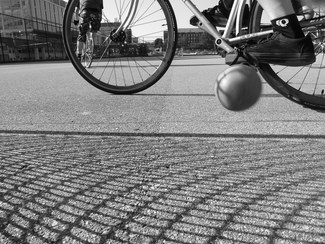
\includegraphics[width=4.25in]{a2bp.jpg} \\[1cm]

Ann Arbor Bike Polo
\small{{\tt http://kula.tproa.net/photos/2010/20100530-bike-polo/}}

\end{center}

\newpage

\thispagestyle{empty}
\vspace*{14cm}
\begin{sideways}
\Large{Thomas L. Kula}
\end{sideways}
\begin{sideways}
\Large{PO Box 980461}
\end{sideways}
\begin{sideways}
\Large{Ypsilanti MI 48198}
\end{sideways}


\end{document}


